가로 $N$칸, 세로 $M$칸으로 이루어진 직사각형 모양의 게임판이 있다. 똑같은 게임말 두 개를 서로 대각선으로 이웃하게 올려두는 방법의 수를 출력하시오.

아래 그림은 $N = 3$, $M = 2$인 경우의 예시이다.
\begin{center}
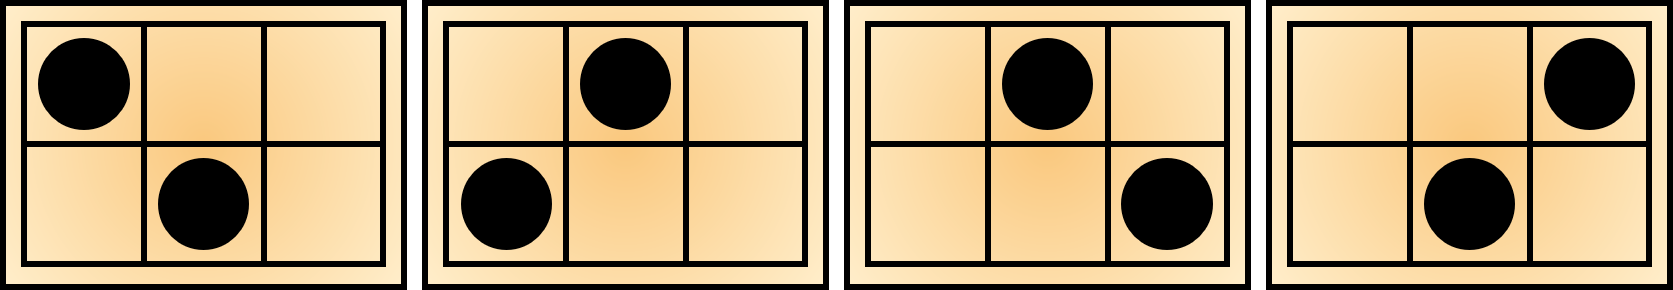
\includegraphics{grid.png}
\end{center}